\chapter{Từ tích phân đường đến hàm truyền và các đỉnh tương tác}

Trước khi chuyển sang danh mục các hạt và các tương tác của chúng, cần làm rõ phép xây dựng trung tâm. Một Lagrangian không chỉ mã hóa các phương trình trường cổ điển. Thông qua tích phân đường, nó còn cung cấp các biên độ để hạt truyền, phân tách, kết hợp và tán xạ. Đây là con đường trực tiếp nhất đi từ lý thuyết trường lượng tử đến các giản đồ Feynman.

\section{Nguyên lý tác dụng cực tiểu cho hạt và trường}

Tích phân đường của Feynman là đối ứng lượng tử của nguyên lý tác dụng cực tiểu. Hãy bắt đầu với một hạt Newton thông thường, có Lagrangian phụ thuộc vào tọa độ và vận tốc của nó,
\begin{equation}
\mathcal{L}=\mathcal{L}(x,\dot{x}),
\end{equation}
và tác dụng gán cho một quỹ đạo là
\begin{equation}
S[x]=\int \mathcal{L}(x,\dot{x})\,dt.
\end{equation}
Mọi quỹ đạo khả dĩ từ một điểm không-thời gian đến một điểm khác đều có một tác dụng, bất kể nó có thỏa mãn các phương trình Newton hay không. Quỹ đạo cổ điển được đặc trưng bởi tính dừng của tác dụng. Theo cách nói truyền thống ``tác dụng cực tiểu'', nó làm cực tiểu tác dụng, mặc dù phát biểu theo tính dừng là tổng quát hơn. Điều kiện dừng suy ra các phương trình vi phân chuyển động cổ điển.

\begin{figure}[htbp]
\centering
\includegraphics[width=0.72\textwidth]{lecture_10_figure_02.png}
\caption{Tích phân tác dụng cho một quỹ đạo hạt.}
\lectureframe{00:02:14}
\end{figure}

Cùng một cấu trúc áp dụng cho một trường cổ điển. Ký hiệu chung mọi trường là \(\phi\). Mật độ Lagrangian địa phương của trường có thể phụ thuộc vào các trường và vào cả các đạo hàm không gian lẫn thời gian của chúng:
\begin{equation}
\mathcal{L}
=\mathcal{L}\!\left(\phi,\frac{\partial\phi}{\partial x^\mu}\right)
=\mathcal{L}(\phi,\partial_\mu\phi).
\end{equation}
Thuyết tương đối đòi hỏi \(\mathcal{L}\) biến đổi như một vô hướng Lorentz. Với yêu cầu đó, các tổ hợp vô hướng được xây dựng từ các trường và các đạo hàm của chúng cung cấp các hạng có thể có trong Lagrangian.

\begin{figure}[htbp]
\centering
\includegraphics[width=0.62\textwidth]{lecture_10_figure_03.png}
\caption{Sự phụ thuộc của Lagrangian trường vào trường và các đạo hàm không-thời gian của nó.}
\lectureframe{00:04:09}
\end{figure}

Đối với một trường, tác dụng được lấy tích phân trên một miền không-thời gian:
\begin{equation}
S[\phi]=\int_{\Omega} d^4x\,\mathcal{L}(\phi,\partial_\mu\phi),
\qquad
d^4x=dt\,dx\,dy\,dz.
\end{equation}
Tác dụng của hạt là một tích phân theo thời gian dọc theo một đường đi. Tác dụng của trường là mật độ Lagrangian được lấy tích phân trên toàn bộ một miền không-thời gian.

Đối ứng của việc cố định hai đầu mút của một đường đi hạt là ấn định toàn bộ cấu hình trường trên một lát thời gian ban đầu và trên một lát thời gian cuối. Nếu trường ban đầu là \(\phi_{\mathrm{i}}(\mathbf{x})\) và trường cuối là \(\phi_{\mathrm{f}}(\mathbf{x})\), thì một lịch sử trường nội suy lấp đầy toàn bộ phiến không-thời gian giữa chúng. Khi dữ liệu biên cho phép một nghiệm nội suy cổ điển, nghiệm đó là một điểm dừng của tác dụng khi các cấu hình biên được giữ cố định.
\editorialnote{Các cấu hình trường đầy đủ tùy ý trên hai lát thời gian không nhất thiết cho phép một nghiệm cổ điển. Vì vậy, phát biểu về tác dụng dừng bị giới hạn ở những dữ liệu biên mà đối với chúng tồn tại một nghiệm nội suy.}

Hình học này là đối tượng tương ứng trong lý thuyết trường của một đường đi hạt.\footnote{Phiến không-thời gian được phục dựng từ hình vẽ vào khoảng 00:04:29.}
\begin{figure}[htbp]
\centering
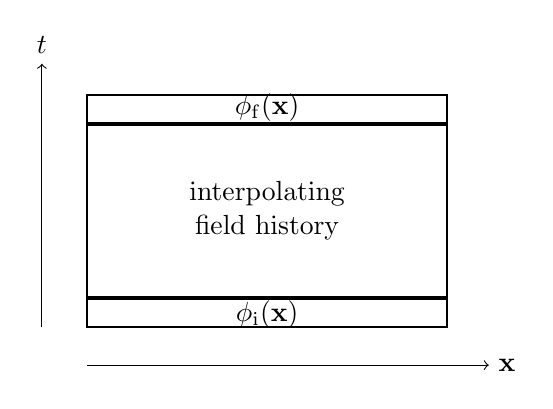
\begin{tikzpicture}[scale=0.88]
\draw[->] (-0.65,0) -- (-0.65,3.8) node[above] {$t$};
\draw[->] (0,-0.55) -- (5.8,-0.55) node[right] {$\mathbf{x}$};
\draw[thick] (0,0) rectangle (5.2,3.35);
\draw[very thick] (0,0.42) -- (5.2,0.42);
\draw[very thick] (0,2.93) -- (5.2,2.93);
\node at (2.6,0.18) {$\phi_{\mathrm{i}}(\mathbf{x})$};
\node at (2.6,3.17) {$\phi_{\mathrm{f}}(\mathbf{x})$};
\node[align=center] at (2.6,1.68) {interpolating\\field history};
\end{tikzpicture}
\caption{Các cấu hình trường ban đầu và cuối cùng giới hạn một miền không-thời gian.}
\end{figure}

\begin{classroomqa}
\lecturetimestamp{00:07:34}
\audiencequestion{Một trường có thể trở lại đúng cùng một giá trị không?}
\lecturerresponse{Có. Không có gì ngăn cản một trường trở lại một giá trị trước đó, cũng như không có gì ngăn cản một tọa độ của hạt trở lại một vị trí trước đó.}
\end{classroomqa}

\begin{classroomqa}
\lecturetimestamp{00:07:46}
\audiencequestion{Tại sao lại nói về các sự kiện không-thời gian hay một quỹ đạo khi dữ liệu biên là các giá trị trường?}
\lecturerresponse{Quỹ đạo hạt được thay bằng một lịch sử trường. Mỗi đầu mút trong không gian trường chính là toàn bộ trường trên một lát thời gian đã chọn, và một lịch sử xác định trường tại mọi điểm trong miền không-thời gian giữa hai lát ấy.}
\end{classroomqa}

Việc đòi hỏi tác dụng dừng đối với trường nội suy tạo ra các phương trình vi phân riêng phần. Tùy theo các trường và Lagrangian, chúng bao gồm những phương trình như phương trình Maxwell và, đối với một tác dụng hấp dẫn, phương trình Einstein. Ở đây không cần đến phép suy diễn biến phân chi tiết; chuỗi quan trọng là
\begin{equation}
\mathcal{L}
\longrightarrow
S[\phi]
\longrightarrow
\text{classical field equations}.
\end{equation}

\section{Phép tổng trên các đường đi hạt của Feynman}

Cơ học lượng tử thay câu hỏi quỹ đạo nào xảy ra bằng một câu hỏi về biên độ. Hãy hình dung đưa một hạt vào tại \((x,t)\), nhắm mắt một lúc, rồi bật một máy dò tại \((x',t')\). Biên độ
\begin{equation}
\mathcal{A}(x,t;x',t')
\end{equation}
là một số phức. Bình phương môđun của nó là xác suất:
\begin{equation}
\begin{aligned}
P(x,t;x',t')
&=\left|\mathcal{A}(x,t;x',t')\right|^2\\
&=\mathcal{A}(x,t;x',t')
\mathcal{A}(x,t;x',t')^*.
\end{aligned}
\end{equation}

Quy tắc của Feynman gán một tác dụng cho mọi đường đi khả dĩ và gắn với nó pha
\begin{equation}
\exp\!\left(-\frac{i}{\hbar}S[x]\right)
=
\exp\!\left[-\frac{i}{\hbar}\int \mathcal{L}(x,\dot{x})\,dt\right].
\end{equation}

\begin{figure}[htbp]
\centering
\includegraphics[width=0.70\textwidth]{lecture_10_figure_04.png}
\caption{Pha phức gắn với một đường đi của hạt.}
\lectureframe{00:11:52}
\end{figure}

Hệ số \(\hbar\) là cần thiết để làm cho số mũ không thứ nguyên.\footnote{Vào lúc 00:11:52, biểu thức trên bảng tự nhiên là \(e^{-i\int\mathcal{L}\,dt}\); hệ số của \(\hbar\) được bổ sung bằng lời tại 00:12:02.} Biên độ chuyển tiếp là tổng của các pha này trên mọi đường đi khả dĩ nối hai đầu mút:
\begin{equation}
\mathcal{A}(x,t;x',t')
=
\sum_{\substack{\text{paths }x(\tau)\\(x,t)\rightarrow(x',t')}}
\exp\!\left(-\frac{i}{\hbar}S[x]\right).
\end{equation}
Ở đây ``đường đi khả dĩ'' không có nghĩa là một nghiệm của các phương trình Newton. Nó có nghĩa là bất kỳ đường đi nào được đưa vào phép tổng. Trong cơ học lượng tử phi tương đối tính, các đường đi tiến về phía trước theo thời gian thay vì vòng lùi ngược lại. Hằng số Planck có thứ nguyên của tác dụng, nên \(S/\hbar\) là không thứ nguyên.

Hàm mũ này là tự nhiên vì các biên độ cho những bước nhỏ liên tiếp nhân với nhau. Nếu một đường đi được chia thành các đoạn liên tiếp, tác dụng cộng lại,
\begin{equation}
S=S_1+S_2+\cdots,
\end{equation}
trong khi các pha nhân với nhau:
\begin{equation}
e^{-iS/\hbar}
=e^{-iS_1/\hbar}e^{-iS_2/\hbar}\cdots.
\end{equation}
Hệ số \(i\) không phải là một thủ thuật ghi chép; nó là một phần của quy tắc cơ học lượng tử.

\begin{classroomqa}
\lecturetimestamp{00:13:27}
\audiencequestion{Hàm mũ có liên hệ với việc nhân các biên độ cho những bước nhỏ liên tiếp không?}
\lecturerresponse{Có. Các biên độ của những bước liên tiếp nhân với nhau, còn các phần tương ứng của tác dụng thì cộng lại.}
\end{classroomqa}

\begin{classroomqa}
\lecturetimestamp{00:13:49}
\audiencequestion{Bản thân phép tổng trên các đường đi có phải là xác suất không?}
\lecturerresponse{Không. Tổng trên các đường đi là một biên độ xác suất nói chung là phức. Nhân nó với liên hợp phức của nó cho ta xác suất.}
\end{classroomqa}

\section{Phép tổng trên các lịch sử trường}

Cách phát biểu này cũng mở rộng sang lý thuyết trường lượng tử, mặc dù cách xây dựng ở đây sẽ vẫn cố ý không nghiêm ngặt. Bắt đầu với một cấu hình trường ban đầu \(\phi(\mathbf{x})\) và một cấu hình cuối được chỉ định riêng rẽ \(\phi'(\mathbf{x})\). Đây là các hàm đầy đủ của không gian, không phải các giá trị tại hai điểm cô lập.

Ta có thể hình dung một thiết bị lý tưởng hóa chuẩn bị trường tại mọi điểm trong không gian, để hệ tiến hóa, rồi về sau đo trường tại mọi điểm. Thiết bị như vậy không hiện thực, nhưng nó nêu câu hỏi khái niệm một cách rõ ràng: biên độ để đi từ cấu hình trường đầy đủ ban đầu sang cấu hình cuối là bao nhiêu?

Mọi lịch sử trường nội suy có thể hình dung đều đóng góp. Với mỗi lịch sử, tính
\begin{equation}
S[\phi]=\int d^4x\,\mathcal{L}(\phi,\partial_\mu\phi)
\end{equation}
và gắn pha tương ứng. Ở mức sơ đồ,
\begin{equation}
\mathcal{A}\!\left[\phi(\mathbf{x})\rightarrow\phi'(\mathbf{x})\right]
=
\sum_{\substack{\text{field histories}\\
\phi_{\mathrm{i}}=\phi,\;\phi_{\mathrm{f}}=\phi'}}
\exp\!\left(-\frac{i}{\hbar}S[\phi]\right).
\end{equation}
Một lịch sử không nhất thiết phải nghiệm các phương trình trường cổ điển. Nó đơn giản chỉ là một phép gán đầy đủ các giá trị trường trên toàn bộ miền không-thời gian xen giữa.

\begin{classroomqa}
\lecturetimestamp{00:17:39}
\audiencequestion{Có vô số lịch sử, và mỗi pha đều có độ lớn bằng 1. Làm sao tổng của chúng có thể hội tụ? Có phải các lịch sử đang được cực tiểu hóa không?}
\lecturerresponse{Các lịch sử được cộng lại, không phải được cực tiểu hóa. Các số hạng là những pha phân bố quanh đường tròn đơn vị, nên chúng có thể triệt tiêu lẫn nhau. Điều này khác với việc cộng vô số số hạng dương được chặn dưới bởi một giá trị khác 0. Các tích phân dao động có thể hội tụ; biểu diễn Fourier của một hàm delta là một ví dụ quen thuộc. Nếu các pha phân bố đều quanh đường tròn, tổng vectơ của chúng sẽ triệt tiêu. Phần lớn các lịch sử triệt tiêu lẫn nhau rất mạnh. Các lịch sử gần một quỹ đạo tác dụng dừng triệt tiêu ít nhất vì ở đó pha biến thiên chậm nhất, và đó là cách giới hạn cổ điển xuất hiện.}
\end{classroomqa}

\editorialnote{Một tích phân đường trong thời gian thực thông thường đòi hỏi một quy tắc hội tụ. Thảo luận về đường tròn đơn vị chỉ đưa ra lập luận triệt tiêu dao động được dùng ở đây, chứ không phải một chứng minh tổng quát về hội tụ.}

Sự triệt tiêu này có thể được hình dung như một tổng vectơ trong mặt phẳng phức.\footnote{Cách dựng đường tròn đơn vị được phục dựng từ phần thảo luận trên bảng ở khoảng 00:18:32--00:20:21.}
\begin{figure}[htbp]
\centering
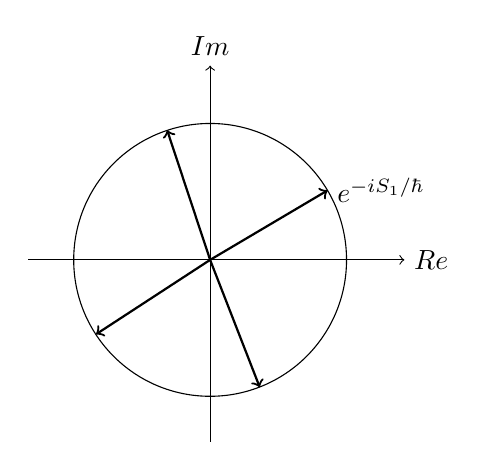
\begin{tikzpicture}[scale=1.05]
\draw[->] (-2.2,0) -- (2.35,0) node[right] {$\operatorname{Re}$};
\draw[->] (0,-2.2) -- (0,2.35) node[above] {$\operatorname{Im}$};
\draw (0,0) circle (1.65);
\draw[thick,->] (0,0) -- (1.42,0.84);
\draw[thick,->] (0,0) -- (-1.38,-0.90);
\draw[thick,->] (0,0) -- (-0.52,1.57);
\draw[thick,->] (0,0) -- (0.60,-1.54);
\node[right] at (1.42,0.84) {$e^{-iS_1/\hbar}$};
\end{tikzpicture}
\caption{Các pha có độ lớn đơn vị có thể triệt tiêu nhau khi hướng của chúng khác nhau.}
\end{figure}

Thật vậy,
\begin{equation}
e^{-iS/\hbar}
=
\cos\!\left(\frac{S}{\hbar}\right)
-i\sin\!\left(\frac{S}{\hbar}\right).
\end{equation}
Mỗi đóng góp là một vectơ đơn vị. Các đóng góp theo các hướng khác nhau có thể trừ nhau cũng như cộng nhau. Gần một điểm dừng của \(S\), các lịch sử lân cận có gần như cùng một pha, nên các đóng góp của chúng tăng cường lẫn nhau hiệu quả hơn. Xa khỏi tác dụng dừng, pha biến thiên nhanh và giao thoa triệt tiêu chiếm ưu thế.

Cấu trúc tích phân đường này làm nền cho về cơ bản toàn bộ lý thuyết trường lượng tử hiện đại. Bước thực hành tiếp theo sẽ được phát biểu chứ không được suy ra. Đây là một lối vào phép tính đã được đơn giản hóa quá mức, nhưng nó làm bộc lộ cách cùng một đối tượng có thể được dùng trong hai ngôn ngữ.

Tính toán một quá trình là tính toán xác suất chuyển tiếp từ ban đầu đến cuối. Một cách mô tả chỉ rõ một cấu hình trường ban đầu và một cấu hình trường cuối. Cách kia chỉ rõ các hạt vào và các hạt ra, tức các lượng tử của một hoặc vài trường. Hai câu hỏi này trông khác nhau, nhưng cả hai đều được tính từ cùng một tích phân đường của lý thuyết trường.

\section{Một dạng không-thời gian rời rạc}

Để cho phép tổng trên các lịch sử trường một ý nghĩa cụ thể, hãy chia không-thời gian thành các ô nhỏ và gán một giá trị trường cho mỗi ô. Giới hạn liên tục đạt tới bằng cách làm kích thước ô co lại, nhưng hiện thời các ô vẫn hữu hạn. Điều này biến phép tổng hình thức trên các hàm thành một phép tổng trên các phép gán số cho các ô mạng.

Một lập luận trực giác trước đó dùng một tích các nhân tử giống \(1+\mathcal{L}_i\), một cho mỗi ô, rồi nhận ra các hạng mô tả sự truyền và va chạm của hạt. Cách dựng này đủ trung tâm để nhắc lại, nhưng nhân tử ấy phải được hiệu chỉnh. Đại lượng nhỏ không phải chính bản thân Lagrangian. Nó là tác dụng chứa trong một ô.

Nếu một ô có thể tích không-thời gian
\begin{equation}
a^4=\Delta t\,\Delta x\,\Delta y\,\Delta z,
\end{equation}
thì tác dụng của nó là
\begin{equation}
A_i=\mathcal{L}_i a^4.
\end{equation}
Vì ô nhỏ nên \(A_i\) là nhỏ. Tạm thời lược bỏ \(\hbar\), nhân tử sơ cấp đã hiệu chỉnh là
\begin{equation}
1-iA_i,
\end{equation}
thay vì \(1+\mathcal{L}_i\).

Với mọi \(\epsilon\) nhỏ,
\begin{equation}
1+\epsilon\simeq e^\epsilon,
\end{equation}
vì
\begin{equation}
e^\epsilon
=1+\epsilon+\frac{\epsilon^2}{2!}
+\frac{\epsilon^3}{3!}+\cdots.
\end{equation}
Do đó, trong hệ đơn vị tạm thời này, \(1-iA_i\) xấp xỉ \(e^{-iA_i}\) đối với một ô đủ nhỏ. Gọn hơn là dùng ngay từ đầu nhân tử hàm mũ chính xác.

\begin{classroomqa}
\lecturetimestamp{00:27:57}
\audiencequestion{Nhân tử hàm mũ có cần một hệ số \(\hbar\) không?}
\lecturerresponse{Có. Nhân tử ô không thứ nguyên ở bậc nhất là \(1-iA_i/\hbar\), và hàm mũ chính xác là \(\exp(-iA_i/\hbar)\). Về sau ta có thể chọn các đơn vị trong đó \(\hbar=1\).}
\end{classroomqa}

Khôi phục \(\hbar\), nhân tử trung gian đã hiệu chỉnh và dạng hàm mũ của nó là
\begin{equation}
1-\frac{i}{\hbar}A_i
\simeq
\exp\!\left(-\frac{i}{\hbar}A_i\right).
\end{equation}

Đối với một lịch sử cố định, thay tích phân không-thời gian bằng tổng các tác dụng của ô:
\begin{equation}
S[\phi]
=\int d^4x\,\mathcal{L}
\;\longrightarrow\;
\sum_i A_i.
\end{equation}
Pha cho lịch sử đó trở thành
\begin{equation}
\exp\!\left(-\frac{i}{\hbar}\sum_i A_i\right).
\end{equation}
Hàm mũ của một tổng là tích của các hàm mũ:
\begin{equation}
\exp\!\left(-\frac{i}{\hbar}\sum_i A_i\right)
=
\prod_i\exp\!\left(-\frac{i}{\hbar}A_i\right).
\end{equation}
Thứ tự thao tác là quan trọng. Trước hết hãy chọn một lịch sử đầy đủ và nhân các trọng số ô của nó. Chỉ sau đó mới lấy tổng trên các lịch sử khác nhau.

Mạng cũng làm cho dữ liệu biên trở nên tường minh.\footnote{Hình ô bàn cờ và các hàng đầu, cuối cố định của nó được phục dựng từ các hình vẽ vào khoảng 00:23:54 và 00:30:49.}
\begin{figure}[htbp]
\centering
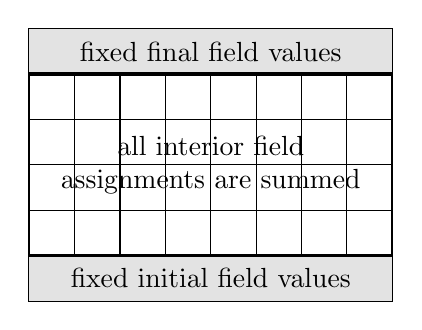
\begin{tikzpicture}[scale=0.72]
\draw[step=0.8,thin] (0,0) grid (6.4,4.8);
\draw[thick] (0,0) rectangle (6.4,4.8);
\fill[gray!22] (0,0) rectangle (6.4,0.8);
\fill[gray!22] (0,4.0) rectangle (6.4,4.8);
\draw[very thick] (0,0.8) -- (6.4,0.8);
\draw[very thick] (0,4.0) -- (6.4,4.0);
\node at (3.2,0.4) {fixed initial field values};
\node at (3.2,4.4) {fixed final field values};
\node[align=center] at (3.2,2.4) {all interior field\\assignments are summed};
\end{tikzpicture}
\caption{Các lịch sử trường rời rạc với các hàng mạng ban đầu và cuối cùng cố định.}
\end{figure}

Hàng đầu tiên xác định cấu hình trường ban đầu, và hàng cuối cùng xác định cấu hình cuối cùng. Mỗi ô bên trong được phép nhận mọi giá trị trường có trong phép rời rạc hóa. Vì vậy biên độ chuyển tiếp có dạng sơ đồ
\begin{equation}
\mathcal{A}\!\left[\phi_{\mathrm{i}}\rightarrow\phi_{\mathrm{f}}\right]
=
\sum_{\{\phi\}_{\mathrm{interior}}}
\prod_i\exp\!\left(-\frac{i}{\hbar}A_i[\phi]\right),
\end{equation}
với hàng đầu và hàng cuối được giữ cố định. Tương đương, với mỗi cách gán ở phần bên trong, ta tính hàm mũ của tác dụng toàn phần rồi cộng đóng góp đó vào các đóng góp từ mọi cách gán khác.

\section{Từ cấu hình trường đến cấu hình hạt}

Cùng một biên độ chuyển tiếp có thể được mô tả theo trường hoặc theo hạt. Thay vì cố định trường trên lát thời gian đầu và cuối, ta có thể chỉ định một tập hợp các lượng tử trường đi vào và một tập hợp các lượng tử trường đi ra, rồi hỏi biên độ nối chúng. Đối tượng đang được tính là như nhau. Chỉ mô tả ở biên là đã thay đổi.

Trường lượng tử chứa các toán tử tạo và hủy. Vì thế các tích của trường tác dụng lên các trạng thái hạt bằng cách tạo ra, hủy đi, hoặc dịch chuyển các lượng tử. Cách đọc theo toán tử này chính là điều biến tích phân đường trên mạng thành một bộ quy tắc hạt.

\begin{classroomqa}
\lecturetimestamp{00:34:11}
\audiencequestion{Các lượng tử trường có nhất thiết có thể được nhận diện là các hạt không?}
\lecturerresponse{Không phải lúc nào cũng theo nghĩa thông thường của những hạt có thể quan sát riêng rẽ. Chẳng hạn, quark là các lượng tử của các trường quark, nhưng hiện tượng giam hãm ngăn không cho một quark cô lập thoát ra và được phát hiện riêng rẽ. Tổng quát hơn, không nhất thiết có sự tương ứng một-một giữa các trường được nêu tên trong một lý thuyết và các loại hạt xuất hiện như những trạng thái quan sát được theo nghĩa thông thường. Một số lý thuyết trường không cho phép sự tương ứng đơn giản đó. Nếu ``particle'' được dùng theo nghĩa rộng để chỉ một lượng tử không thể chia nhỏ mang năng lượng và các số lượng tử khác, thì sự phân biệt có thể phần nào trở thành vấn đề thuật ngữ.}
\end{classroomqa}

\editorialnote{Mệnh đề về ghép yếu trong bản nguồn tại 00:35:45--00:36:08 mơ hồ về mặt ngữ pháp và ở đây được để nguyên, không giải quyết. Khẳng định chắc chắn là các nhãn trường và các loại hạt quan sát được theo nghĩa thông thường không nhất thiết tương ứng một-một.}

Bản thân tổng trên mạng vẫn chạy qua các giá trị trường. Nó không bị giới hạn ở những cấu hình giống các nghiệm cổ điển trơn.

\begin{classroomqa}
\lecturetimestamp{00:36:44}
\audiencequestion{Các lịch sử trường có phải liên tục, hoặc ít nhất xấp xỉ liên tục, không?}
\lecturerresponse{Không. Trên một mạng rời rạc, các ô lân cận đơn giản chỉ mang các giá trị trường, và mọi cách gán đều được đưa vào tổng. Không có sự giới hạn vào các lịch sử xấp xỉ liên tục. Các trường lượng tử dao động mạnh; các lịch sử điển hình không phải là các trường cổ điển trơn.}
\end{classroomqa}

Các biến được gán độc lập là các trường tại những nút hoặc ô của mạng. Các đạo hàm của chúng được lấy từ hiệu giữa các giá trị lân cận.

\begin{classroomqa}
\lecturetimestamp{00:37:56}
\audiencequestion{Các trường và các đạo hàm của chúng có được gán các giá trị độc lập không?}
\lecturerresponse{Không. Các giá trị trường được gán tại các nút. Sau đó một đạo hàm được tái dựng từ hiệu giữa các giá trị trường lân cận. Có thể dùng những quy ước sai phân hữu hạn khác nhau, nhưng các đạo hàm không phải là những biến độc lập bổ sung.}
\end{classroomqa}

Vì vậy, với khoảng cách mạng \(a\), ta có thể viết một cách sơ đồ
\begin{equation}
\partial_\mu\phi(x)
\longrightarrow
\frac{\phi(x+a\hat\mu)-\phi(x)}{a}.
\end{equation}
Bản thân trục giá trị trường cũng có thể được chia thành các khoảng nhỏ, để lại một tập đếm được các giá trị khả dĩ tại mỗi nút.

\begin{classroomqa}
\lecturetimestamp{00:38:53}
\audiencequestion{Điều gì thay đổi khi có nhiều hơn một trường?}
\lecturerresponse{Tại mỗi nút, ta gán một giá trị cho từng trường, và tổng chạy qua mọi cách gán như vậy.}
\end{classroomqa}

Không nên nhầm một trường nhận giá trị phức với một hàm giải tích của biến phức. Tính giải tích là một điều kiện trơn đặc biệt mạnh. Các lịch sử trong một tích phân đường trường không cần tuân theo nó và, nói chung, thậm chí còn không xấp xỉ trơn.

\begin{classroomqa}
\lecturetimestamp{00:39:07}
\audiencequestion{Nếu các trường nhận giá trị phức, thì các giá trị của chúng có phải thỏa mãn các điều kiện trơn mà các hàm giải tích tuân theo không?}
\lecturerresponse{Không. Nhận giá trị phức không có nghĩa là giải tích. Lý thuyết hàm giải tích xét một lớp hàm cực kỳ trơn và bị ràng buộc chặt chẽ. Các lịch sử trường được cộng ở đây không cần là các hàm giải tích của vị trí; các lịch sử điển hình rất bất quy tắc và có thể được xem là rất gián đoạn trong giới hạn liên tục.}
\end{classroomqa}

Phép tính thu được trông rất ghê gớm. Ngay cả sau khi không-thời gian và các giá trị trường đã được rời rạc hóa, vẫn có thể có một số lượng khổng lồ các cách gán cần lấy mẫu.

\begin{classroomqa}
\lecturetimestamp{00:40:04}
\audiencequestion{Làm sao máy tính biết cần lấy mẫu bao nhiêu cách gán trên mạng, hoặc khi nào phép tính đã hội tụ?}
\lecturerresponse{Câu hỏi đó thuộc về lý thuyết chuẩn trên mạng, hay tổng quát hơn là lý thuyết trường lượng tử trên mạng. Đến nay đây là một lĩnh vực tính toán hiệu quả. Tôi có tham gia ngay từ buổi đầu trong việc thiết lập các quy tắc cho lý thuyết chuẩn trên mạng, chứ không tham gia vào công nghệ máy tính về sau. Việc đặt ra các quy tắc mất khoảng 3 tuần; phát triển công nghệ để tính được những thứ này mất cỡ 30 năm. Phần lớn kinh nghiệm thực hành đến từ cơ học thống kê, nơi các hàm phân hoạch cũng thu được bằng cách cộng qua các cấu hình của một mạng---chẳng hạn, xét xem một nút trong tinh thể có bị chiếm hay không. Việc xác định đã lấy mẫu đủ cấu hình hay chưa là một vấn đề kỹ thuật. Các chuyên gia biết---hoặc nghĩ rằng họ biết---khi nào phép tính được kiểm soát, và các phép tính thu được phù hợp với thí nghiệm.}
\end{classroomqa}

Các quy tắc ở mức khái niệm cho lý thuyết chuẩn trên mạng xuất hiện khá nhanh; công nghệ cần thiết để tính toán với chúng thì mất lâu hơn nhiều. Bàn cờ không chỉ đơn thuần là một phép so sánh. Nó còn là điểm khởi đầu của một phương pháp tính toán thực tiễn.

\section{Các hạng bậc hai và sự lan truyền của hạt}

Bây giờ hãy trở lại cách diễn giải theo toán tử của các trường. Với hai nút lân cận \(x\) và \(x'\), tích
\begin{equation}
\phi(x)\phi(x')
\end{equation}
trong một phần tử ma trận một-hạt thích hợp có thể cung cấp sự hủy một hạt tại một nút và sự tạo ra nó ở nút kia. Vì vậy, trong sector một-hạt đó, nó có thể được hình dung như một bước nhảy qua một liên kết. Đó là một cách đọc của tích toán tử, chứ không phải nghĩa duy nhất của nó.

Các hạng chịu trách nhiệm cho những liên kết như thế là các hạng đạo hàm. Nói chính xác, chúng gắn không phải với một ô mà với một cặp lân cận. Chẳng hạn, một đạo hàm theo thời gian trở thành
\begin{equation}
\partial_t\phi(t,\mathbf{x})
\longrightarrow
\frac{\phi(t+a,\mathbf{x})-\phi(t,\mathbf{x})}{a},
\end{equation}
và một đạo hàm theo không gian được xử lý theo cùng cách dọc theo một liên kết không gian.

\begin{classroomqa}
\lecturetimestamp{00:44:39}
\audiencequestion{Các Lagrangian đang bàn ở đây có chứa đạo hàm bậc hai không?}
\lecturerresponse{Các lý thuyết thông thường đang được xét ở đây được viết với các đạo hàm bậc nhất. Vì thế các phiên bản trên mạng của chúng dùng các sai phân bậc nhất giữa những nút lân cận.}
\end{classroomqa}

Bình phương một sai phân bậc nhất tạo ra cả các hạng cùng nút lẫn một hạng chéo giữa hai nút lân cận:
\begin{align}
\frac{1}{2}\bigl[\phi(x)-\phi(x')\bigr]^2
&=
\frac{1}{2}\phi(x)^2
+\frac{1}{2}\phi(x')^2
-\phi(x)\phi(x').
\end{align}
Hạng chéo có thể cung cấp sự chuyển từ nút này sang nút kia. Hai số hạng bình phương là các hạng cùng nút. Các hạng bậc hai theo đạo hàm là các hạng động năng, và chính các hạng chéo lân cận của chúng sẽ được dùng trước tiên để xây dựng sự lan truyền.

Để tách riêng phần tổ hợp, hãy gom các tích giữa các nút lân cận vào
\begin{equation}
K=\sum_{\langle x,x'\rangle}\phi(x)\phi(x').
\end{equation}
Nhân tử tương ứng trong trọng số của tích phân đường được viết một cách sơ đồ là
\begin{equation}
e^{-iK}.
\end{equation}
\editorialnote{Trong nhân tử mạng mang tính sơ đồ này, các lũy thừa của khoảng cách mạng, \(\hbar\), các dấu của metric, các hằng số chuẩn hóa và các hệ số của các liên kết đều được lược bỏ.}
Khai triển của nó là
\begin{equation}
e^{-iK}
=1-iK-\frac{1}{2!}K^2+\frac{i}{3!}K^3+\cdots,
\end{equation}
hoặc, khi viết tường minh các tổng trên các cặp lân cận,
\begin{align}
e^{-iK}
={}&1
-i\sum_{\langle x,x'\rangle}\phi(x)\phi(x')
\nonumber\\
&-\frac{1}{2!}
\sum_{\langle x,x'\rangle}
\sum_{\langle y,y'\rangle}
\phi(x)\phi(x')\phi(y)\phi(y')
+\cdots .
\end{align}
Mỗi nhân tử chọn độc lập một cặp lân cận.

Các giản đồ hạt tuân theo một quy tắc không có đầu treo. Một đầu mút lộ ra chỉ được phép ở chỗ điều kiện biên chèn tường minh một hạt vào lát ban đầu hoặc lấy đi một hạt ở lát cuối cùng. Một liên kết cô lập ở phần bên trong có các đầu không khớp và không biểu diễn một đóng góp hoàn chỉnh cho chuyển tiếp đã được chỉ định. Các đầu trong của các liên kết phải nối với nhau.

Trước hết hãy xét một mạng chỉ cao hai lớp thời gian. Nếu trạng thái ban đầu chèn một hạt tại \(x\) và trạng thái cuối cùng lấy nó đi tại điểm lân cận \(x'\), thì hạng bậc nhất có thể nối hai phép chèn ở biên:
\begin{equation}
x\longrightarrow x',
\qquad
\mathcal{A}_{\text{one link}}\sim -i.
\end{equation}
Hệ số \(-i\) chỉ là hệ số trong khai triển sơ đồ này; các nhân tử mạng và chuẩn hóa đã lược bỏ vẫn được ngầm hiểu.

\begin{classroomqa}
\lecturetimestamp{00:52:16}
\audiencequestion{Hạng một-liên-kết bậc nhất có chỉ đóng góp khi các nút đầu và cuối hữu quan kề nhau không?}
\lecturerresponse{Có. Hạng đó chọn một cặp lân cận, nên nó chỉ có thể nối các nút biên ấy khi chúng là láng giềng. Sự lan truyền xa hơn đến từ các tích bậc cao hơn.}
\end{classroomqa}

Ở bậc hai, hai nhân tử được lấy tổng độc lập trên các cặp lân cận:
\begin{equation}
K^2
=
\sum_{\langle x,x'\rangle}
\sum_{\langle y,y'\rangle}
\phi(x)\phi(x')\phi(y)\phi(y').
\end{equation}

\begin{classroomqa}
\lecturetimestamp{00:52:40}
\audiencequestion{Cặp lân cận thứ hai có bắt buộc phải kề với cặp được nhân tử thứ nhất chọn không?}
\lecturerresponse{Không. Mỗi nhân tử chọn độc lập một cặp lân cận. Hai cặp có thể chung một nút, có thể hoàn toàn tách rời, hoặc thậm chí có thể chính là cùng một cặp. Tổng bao gồm mọi khả năng.}
\end{classroomqa}

Đối với một hạt lan truyền qua ba lớp thời gian, lựa chọn bậc hai hữu ích có một nút trung gian chung:
\begin{equation}
\bigl[\phi(x_0)\phi(x_1)\bigr]
\bigl[\phi(x_1)\phi(x_2)\bigr],
\qquad
x_0\longrightarrow x_1\longrightarrow x_2.
\end{equation}
Đầu cuối của liên kết thứ nhất nối với điểm đầu của liên kết thứ hai. Chỉ đầu mút ban đầu tại \(x_0\) và đầu mút cuối cùng tại \(x_2\) còn lộ ra, nên hạng này đóng góp vào chuyển tiếp một-hạt cần tìm. Trong hàm mũ sơ đồ, hệ số của nó là
\begin{equation}
-\frac{1}{2!}.
\end{equation}

Các lựa chọn cũng có thể tạo thành những bước nhảy tách rời.\footnote{Các giản đồ liên kết được tái dựng từ đoạn tại 00:49:18--00:55:12.}
\begin{figure}[htbp]
\centering
\resizebox{\linewidth}{!}{%
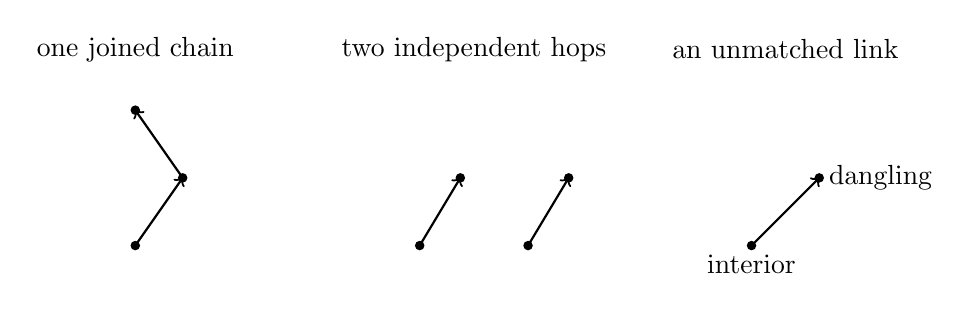
\begin{tikzpicture}[scale=0.86]
\node at (0,2.9) {one joined chain};
\fill (0,0) circle (2pt);
\fill (0.7,1.0) circle (2pt);
\fill (0,2.0) circle (2pt);
\draw[thick,->] (0,0) -- (0.7,1.0);
\draw[thick,->] (0.7,1.0) -- (0,2.0);

\begin{scope}[xshift=4.2cm]
\node at (0.8,2.9) {two independent hops};
\fill (0,0) circle (2pt);
\fill (0.6,1.0) circle (2pt);
\fill (1.6,0) circle (2pt);
\fill (2.2,1.0) circle (2pt);
\draw[thick,->] (0,0) -- (0.6,1.0);
\draw[thick,->] (1.6,0) -- (2.2,1.0);
\end{scope}

\begin{scope}[xshift=9.1cm]
\node at (0.5,2.9) {an unmatched link};
\fill (0,0) circle (2pt);
\fill (1.0,1.0) circle (2pt);
\draw[thick,->] (0,0) -- (1.0,1.0);
\node[below] at (0,0) {interior};
\node[right] at (1.0,1.0) {dangling};
\end{scope}
\end{tikzpicture}%
}
\caption{Các lựa chọn liên kết lân cận kiểu nối liền, độc lập và không khớp.}
\end{figure}

Ngay ở bậc này đã có thể có hơn một lộ trình. Với một độ dời gồm một bước mạng theo thời gian và một bước theo không gian, hai thứ tự
\begin{align}
x
&\longrightarrow x+\hat t
\longrightarrow x+\hat t+\hat s,\\
x
&\longrightarrow x+\hat s
\longrightarrow x+\hat s+\hat t
\end{align}
đi tới cùng một điểm cuối.

\begin{classroomqa}
\lecturetimestamp{00:55:53}
\audiencequestion{Có một đường đi hai bước nào khác tới cùng điểm cuối chéo đó không?}
\lecturerresponse{Có. Ta có thể đi bước thời gian trước và bước không gian sau, hoặc đi theo thứ tự ngược lại. Cả hai lộ trình đều đóng góp vào cùng một biên độ chuyển tiếp.}
\end{classroomqa}

Không có lý do gì phải dừng ở hai liên kết. Hạng bậc ba cung cấp các chuỗi gồm ba liên kết lân cận. Một lộ trình có thể tiến thẳng, có thể đi vòng, hoặc có thể đi lệch ra rồi quay lại trước khi đến điểm cuối cùng. Các bậc còn cao hơn nữa bao gồm những vòng tránh dài hơn và những lần lùi lại lặp đi lặp lại. Vì vậy, khai triển đến bậc tùy ý tạo ra một đóng góp cho mọi lộ trình được ghép từ các liên kết cục bộ. Biên độ từ điểm này đến điểm kia là tổng của tất cả chúng, với các hệ số chứa các lũy thừa thích hợp của \(i\) và các giai thừa:
\begin{equation}
\begin{gathered}
\mathcal{A}(x_{\mathrm{in}}\to x_{\mathrm{out}})
=
\sum_{\text{joined lattice routes }r}c_r,
\\
c_r\ \hbox{read from the exponential expansion}.
\end{gathered}
\end{equation}
Các hệ số nói chung là phức, nên biên độ thu được là phức.

Sự lan truyền tương đối tính bổ sung một khả năng khác. Một lộ trình có thể đi cả lên lẫn xuống theo hướng thời gian, và nó có thể đi qua cùng một liên kết nhiều lần.

\begin{classroomqa}
\lecturetimestamp{00:58:47}
\audiencequestion{Một đường đi có thể đi qua đi lại mãi qua cùng hai ô không?}
\lecturerresponse{Có. Các lần đi lặp lại đều được tính đến, và trong khai triển tương đối tính lộ trình cũng có thể đi ngược thời gian.}
\end{classroomqa}

Một đoạn đi ngược theo thời gian cho phép hai cách đọc trên hình tương đương. Có thể xem nó như một đường hạt chạy lùi theo thời gian. Hoặc, nếu chỉ lần theo thời gian về phía trước: một cặp hạt--phản hạt được tạo ra, hạt tiếp tục đi tới, còn phản hạt về sau gặp và hủy cặp với hạt ban đầu. Cùng một đường liên thông mã hóa cả hai mô tả.\footnote{Hai cách đọc này bám theo hình vẽ và phần giải thích tại 00:59:00--00:59:51.}

\begin{figure}[htbp]
\centering
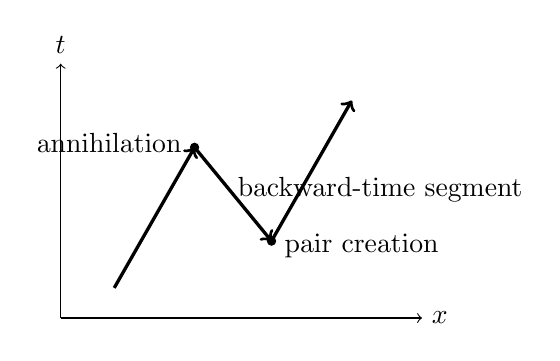
\begin{tikzpicture}[scale=0.85]
\draw[->] (0,0) -- (0,3.8) node[above] {$t$};
\draw[->] (0,0) -- (5.4,0) node[right] {$x$};
\draw[very thick,->] (0.8,0.45) -- (2.0,2.55);
\draw[very thick,->] (2.0,2.55) -- (3.15,1.15);
\draw[very thick,->] (3.15,1.15) -- (4.35,3.25);
\fill (2.0,2.55) circle (2pt);
\fill (3.15,1.15) circle (2pt);
\node[left] at (1.95,2.62) {annihilation};
\node[right] at (3.20,1.08) {pair creation};
\node[right] at (2.50,1.92) {backward-time segment};
\end{tikzpicture}
\caption{Một đoạn đi ngược theo thời gian, khi đọc theo chiều tiến của thời gian, tương ứng với sự tạo cặp và hủy cặp.}
\end{figure}

Các giai thừa xuất hiện ở bậc cao kiểm soát chuỗi lũy thừa của hàm mũ, nhưng điều đó không đồng nghĩa với việc kiểm soát toàn bộ tổng trên các cấu hình trường.

\begin{classroomqa}
\lecturetimestamp{01:00:00}
\audiencequestion{Các thừa số \(1/n!\) có bảo đảm sự hội tụ không?}
\lecturerresponse{Chúng bảo đảm sự hội tụ của chuỗi mũ đối với một đối số cố định. Tự bản thân chúng không bảo đảm sự hội tụ của tổng riêng biệt trên mọi cấu hình trường. Đó là những câu hỏi khác nhau. Trên một mạng hữu hạn với một tập hữu hạn các giá trị trường đã được rời rạc hóa, số cấu hình là hữu hạn, nhưng các giới hạn liên tục và thể tích vô hạn đòi hỏi sự khống chế bổ sung.}
\end{classroomqa}

\section{Tích trên một liên kết, nhiều cách đọc theo hạt}

Tích bậc hai không chỉ chứa sự lan truyền của một hạt. Khi hai cặp kề nhau của nó chung một đầu mút, nó có thể đưa một hạt đi qua một chuỗi hai liên kết:
\begin{equation}
\bigl[\phi(x_0)\phi(x_1)\bigr]
\bigl[\phi(x_1)\phi(x_2)\bigr].
\end{equation}
Khi các cặp được chọn tách rời nhau, cùng hạng bậc hai đó có thể đưa hai hạt đi, mỗi hạt qua một liên kết.\footnote{Sự so sánh giữa sự lan truyền một hạt và hai bước nhảy một liên kết độc lập được phục dựng từ phần thảo luận trên bảng tại 01:00:46--01:02:34.}
\begin{equation}
\bigl[\phi(x_0)\phi(x_1)\bigr]
\bigl[\phi(y_0)\phi(y_1)\bigr],
\qquad x_0\neq y_0.
\end{equation}
Thừa số thứ nhất vận chuyển một hạt, còn thừa số thứ hai vận chuyển một hạt khác. Vì vậy, khai triển mạng bậc hai chứa các biên độ lan truyền trong mọi sector nhiều hạt. Cùng một bậc đại số có thể mô tả một đường đi liên thông dài hơn hoặc vài đường đi ngắn hơn nhưng rời nhau.

Đây là rất nhiều thông tin, nhưng nó chưa phải là một đỉnh tương tác đúng nghĩa. Chỉ với các hạng lan truyền bậc hai, các đường hạt liên thông không tách thành một số đường khác. Các quá trình làm thay đổi số hạt đòi hỏi những tương tác bổ sung, mặc dù các tích toán tử địa phương có thể cho phép nhiều cách đọc theo tạo và hủy.

\begin{classroomqa}
\lecturetimestamp{01:03:30}
\audiencequestion{Một electron và một positron có thể hủy nhau mà hoàn toàn không để lại hạt nào hay không?}
\lecturerresponse{Một đóng góp với năng lượng vào khác không và không có trạng thái cuối nào mang năng lượng là vi phạm bảo toàn năng lượng. Khi lấy tổng trên các vị trí không-thời gian khả dĩ của nó, các biên độ triệt tiêu nhau. Sự hủy electron--positron có thể xảy ra khi một trường khác mang năng lượng đi---ví dụ khi tạo ra các lượng tử điện từ.}
\end{classroomqa}

\editorialnote{Đoạn trao đổi rút gọn này đi thẳng từ bước nhảy bậc hai đến sự hủy electron--positron. Điểm phân biệt chắc chắn ở đây là các hạng bậc hai cung cấp sự lan truyền tự do, còn sự hủy vật lý đòi hỏi một tương tác với trường khác; biên độ không có đầu ra bị triệt tiêu bởi bảo toàn năng lượng.}

Vì thế, các hạng đạo hàm làm được rất nhiều việc, nhưng không phải mọi việc. Các hạng tiếp theo trong Lagrangian được xác định bởi các tính chất và tương tác của các trường đã được quan sát bằng thực nghiệm.

\section{Hạng khối lượng}

Đối với một trường vô hướng, cấu trúc đạo hàm đang xét có mẫu dấu Lorentz dạng sơ đồ
\begin{equation}
\mathcal{L}_{\mathrm{kin}}
\sim
\frac{1}{2}\left[
(\partial_t\phi)^2
-(\partial_x\phi)^2
-(\partial_y\phi)^2
-(\partial_z\phi)^2
\right].
\end{equation}
Cách viết này xác định cấu trúc thời gian trừ không gian liên quan đến thảo luận; các quy ước về dấu tổng thể và chuẩn hóa được để ngầm hiểu.

Lagrangian cũng có thể chứa các lũy thừa của trường không có đạo hàm. Ví dụ bậc hai có dạng
\begin{equation}
\text{mass term}\ \propto\ \frac{1}{2}m^2\phi^2,
\end{equation}
trong đó \(m^2\) được nhận diện là hệ số khối lượng.\editorialnote{Nguồn không ấn định quy ước dấu tổng thể cho Lagrangian vô hướng đầy đủ trong đoạn này.} Trong cách đọc hạt sơ đồ, hạng này hủy một hạt rồi tái tạo nó ngay tại cùng một nút mạng. Nó không làm dời hạt. Nó chèn một thừa số tại cùng nút vào một đường đi:
\begin{equation}
\text{particle at }x
\longrightarrow
\boxed{m^2\phi(x)^2}
\longrightarrow
\text{particle still at }x.
\end{equation}
Mỗi lần một phép chèn như vậy tác dụng, đường đi nhận thêm một thừa số tỉ lệ với \(m^2\).

Nếu chỉ giữ lại các hạng đạo hàm, sự lan truyền thu được trong khai triển sơ đồ này là lý thuyết không khối lượng. Đối với một trường có khối lượng, một đường đi có thể bao gồm một số bất kỳ các phép chèn khối lượng tại cùng nút giữa các hạng nhảy của nó. Hạng khối lượng làm thay đổi các trọng số tương đối của những đường đi để hàm truyền thu được mang khối lượng của hạt.

\section{Các hạng bậc ba và các lịch sử tách--nhập lại}

Hạng khối lượng làm thay đổi trọng số của một đường đi mà không di chuyển hạt. Hành vi thú vị hơn bắt đầu với các hạng có bậc lớn hơn hai. Xét một tương tác bậc ba,
\begin{equation}
\mathcal{L}_{\mathrm{int}}=g_3\phi^3.
\end{equation}
Tại một ô mạng, ba thừa số trường có bốn cách đọc theo hạt:
\begin{equation}
1\longrightarrow 2,
\qquad
2\longrightarrow 1,
\qquad
0\longrightarrow 3,
\qquad
3\longrightarrow 0.
\end{equation}
Vì vậy, một thừa số bậc ba có thể hủy một hạt và tạo ra hai, hủy hai và tạo ra một, tạo ra ba, hoặc hủy ba.

Các thừa số cặp kề nhau bậc hai vẫn cung cấp sự lan truyền. Một dãy của chúng có thể đưa một hạt tới một ô, một thừa số bậc ba tại ô đó có thể hấp thụ nó và phát ra hai hạt, và các thừa số bậc hai tiếp theo có thể mang hai hạt ấy đi. Điều này đóng góp vào một biên độ với một hạt vào và hai hạt ra.\footnote{Hình học mạng được phục dựng từ hình vẽ tại 01:08:48--01:09:42.}

\begin{figure}[htbp]
\centering
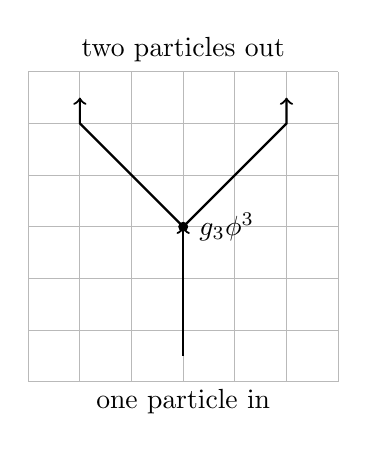
\begin{tikzpicture}[scale=0.82]
\draw[step=0.8,gray!55,thin] (0,0) grid (4.8,4.8);
\draw[thick,->] (2.4,0.4) -- (2.4,1.2) -- (2.4,2.0) -- (2.4,2.4);
\fill (2.4,2.4) circle (2.2pt);
\draw[thick,->] (2.4,2.4) -- (1.6,3.2) -- (0.8,4.0) -- (0.8,4.4);
\draw[thick,->] (2.4,2.4) -- (3.2,3.2) -- (4.0,4.0) -- (4.0,4.4);
\node[right] at (2.5,2.4) {$g_3\phi^3$};
\node at (2.4,-0.3) {one particle in};
\node at (2.4,5.15) {two particles out};
\end{tikzpicture}
\caption{Các thừa số bậc hai lan truyền một hạt vào một đỉnh tách bậc ba và lan truyền các hạt đi ra khỏi đỉnh đó.}
\end{figure}

Ngay cả một biên độ có một hạt ở cả trạng thái đầu lẫn trạng thái cuối cũng không còn chỉ đơn thuần là tổng của những đường đi đơn lẻ không đứt quãng. Một đóng góp là sự lan truyền trực tiếp bởi một chuỗi bước nhảy bậc hai. Một đóng góp khác chứa hai thừa số bậc ba: hạt tách thành hai và về sau hai hạt ấy nhập lại. Vì vậy, trạng thái trung gian có thể chứa nhiều hạt hơn trạng thái ngoài.\footnote{Hai khả năng này được phục dựng từ hình vẽ tại 01:09:44--01:11:36.}

\begin{figure}[htbp]
\centering
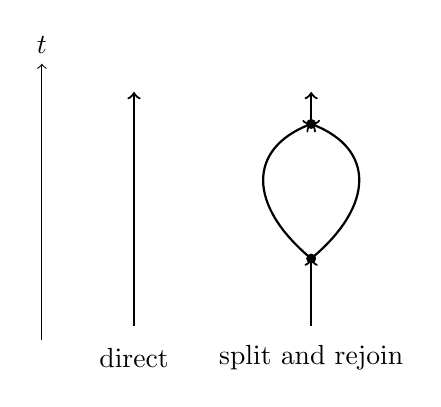
\begin{tikzpicture}[scale=0.9]
\draw[->] (-0.7,0) -- (-0.7,3.9) node[above] {$t$};
\draw[thick,->] (0.6,0.2) -- (0.6,3.5);
\node at (0.6,-0.25) {direct};
\draw[thick,->] (3.1,0.2) -- (3.1,1.15);
\fill (3.1,1.15) circle (2pt);
\draw[thick,->] (3.1,1.15) .. controls (2.2,1.9) and (2.2,2.7) .. (3.1,3.05);
\draw[thick,->] (3.1,1.15) .. controls (4.0,1.9) and (4.0,2.7) .. (3.1,3.05);
\fill (3.1,3.05) circle (2pt);
\draw[thick,->] (3.1,3.05) -- (3.1,3.5);
\node at (3.1,-0.25) {split and rejoin};
\end{tikzpicture}
\caption{Sự lan truyền trực tiếp và một đóng góp tách--nhập lại vào cùng một biên độ một hạt.}
\end{figure}

Trong điện động lực học, ví dụ tương ứng là một electron phát ra một photon rồi về sau hấp thụ lại nó. Lịch sử phát rồi tái hấp thụ đó là một phần của biên độ để electron lan truyền từ điểm này sang điểm khác. Các bậc cao hơn chứa nhiều lần phát và hấp thụ. Một photon có thể chuyển thành một cặp electron--positron, và electron cùng positron trong cặp trung gian đó bản thân chúng cũng có thể trao đổi một photon. Không có gì đòi hỏi thành phần hạt trung gian phải đơn giản chỉ vì thành phần hạt ban đầu và cuối cùng là đơn giản.\footnote{Các ví dụ trong phần phục dựng sau đây xuất hiện tại 01:11:22--01:12:34.}

\begin{figure}[htbp]
\centering
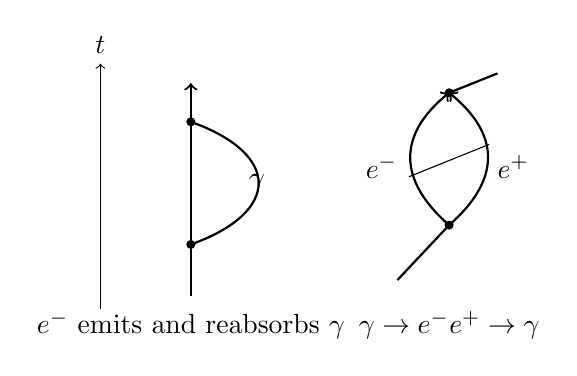
\begin{tikzpicture}[scale=0.82]
\draw[->] (-0.6,0) -- (-0.6,3.8) node[above] {$t$};
\draw[thick,->] (0.8,0.2) -- (0.8,3.5);
\fill (0.8,1.0) circle (2pt);
\fill (0.8,2.9) circle (2pt);
\draw[thick] (0.8,1.0) .. controls (2.2,1.5) and (2.2,2.4) .. (0.8,2.9);
\node[right] at (1.55,1.95) {$\gamma$};
\node at (0.8,-0.25) {$e^-$ emits and reabsorbs $\gamma$};
\draw[thick] (4.0,0.45) -- (4.8,1.3);
\fill (4.8,1.3) circle (2pt);
\draw[thick,->] (4.8,1.3) .. controls (4.0,2.0) and (4.0,2.7) .. (4.8,3.35);
\draw[thick,->] (4.8,1.3) .. controls (5.6,2.0) and (5.6,2.7) .. (4.8,3.35);
\fill (4.8,3.35) circle (2pt);
\draw[thick] (4.8,3.35) -- (5.55,3.65);
\draw[thin] (4.18,2.05) -- (5.42,2.55);
\node[left] at (4.15,2.2) {$e^-$};
\node[right] at (5.4,2.2) {$e^+$};
\node at (4.8,-0.25) {$\gamma\to e^-e^+\to\gamma$};
\end{tikzpicture}
\caption{Một đóng góp trong đó electron phát ra rồi tái hấp thụ photon, và một lịch sử photon chứa một cặp electron--positron.}
\end{figure}

Mỗi lịch sử như vậy xuất phát từ một tích xác định của các hạng trong khai triển của hàm mũ. Hệ số của nó mang lũy thừa thích hợp của \(i\), một giai thừa từ chuỗi mũ, và các hằng số ghép gắn với các đỉnh của nó. Hệ số ấy cho đóng góp của lịch sử đó, nhưng biên độ cho các trạng thái đầu và cuối đã chỉ rõ là tổng của mọi lịch sử có cùng các trạng thái ngoài ấy.

\begin{classroomqa}
\lecturetimestamp{01:13:18}
\audiencequestion{Có phải cùng một quá trình tổng thể có thể xảy ra theo nhiều lịch sử khác nhau, để tất cả chúng đều đóng góp vào biên độ của nó không?}
\lecturerresponse{Có. Biên độ của quá trình được thu được từ tất cả các lịch sử khác nhau nối cùng trạng thái đầu với cùng trạng thái cuối.}
\end{classroomqa}

Vì vậy có hai cách tương đương để tổ chức lý thuyết trường lượng tử. Trong mô tả trường, ta chỉ định một cấu hình trường ban đầu và một cấu hình trường cuối rồi lấy tổng trên mọi lịch sử trường xen giữa. Trong mô tả hạt, trường được phân giải thành các lượng tử: ta chỉ định thành phần hạt đi vào và thành phần hạt đi ra rồi lấy tổng trên mọi lịch sử hạt nối chúng. Cùng một Lagrangian chi phối cả hai mô tả.

\section{Các hạng bậc bốn, các định luật bảo toàn và các hằng số ghép}

Một tương tác bậc bốn,
\begin{equation}
\mathcal{L}_{\mathrm{int}}=g_4\phi^4,
\end{equation}
có bốn thừa số trường tại một điểm. Các cách đọc theo hạt cục bộ của nó bao gồm
\begin{equation}
\begin{gathered}
2\longrightarrow2,
\qquad
1\longrightarrow3,
\qquad
3\longrightarrow1,\\
0\longrightarrow4,
\qquad
4\longrightarrow0.
\end{gathered}
\end{equation}
Vì vậy, một đỉnh bốn chân duy nhất có thể mô tả tán xạ hai hạt, một hạt tách thành ba, ba nhập thành một, hoặc cả bốn chân đều hướng ra ngoài hay hướng vào trong.\footnote{Các định hướng này được phục dựng từ hình vẽ tại 01:14:28--01:15:18.}

\begin{figure}[htbp]
\centering
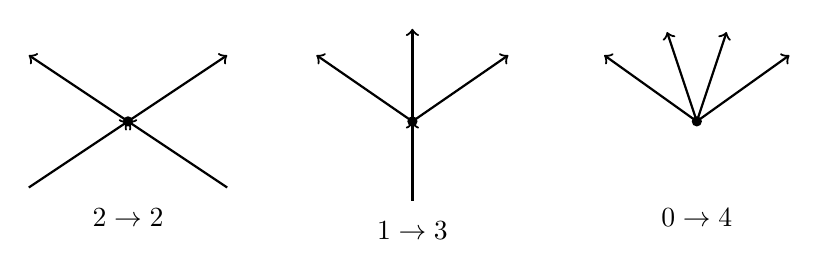
\begin{tikzpicture}[scale=0.84]
\fill (0,0) circle (2.2pt);
\draw[thick,->] (-1.5,-1.0) -- (0,0);
\draw[thick,->] (1.5,-1.0) -- (0,0);
\draw[thick,->] (0,0) -- (-1.5,1.0);
\draw[thick,->] (0,0) -- (1.5,1.0);
\node at (0,-1.45) {$2\to2$};
\begin{scope}[xshift=4.3cm]
\fill (0,0) circle (2.2pt);
\draw[thick,->] (0,-1.2) -- (0,0);
\draw[thick,->] (0,0) -- (-1.45,1.0);
\draw[thick,->] (0,0) -- (0,1.4);
\draw[thick,->] (0,0) -- (1.45,1.0);
\node at (0,-1.65) {$1\to3$};
\end{scope}
\begin{scope}[xshift=8.6cm]
\fill (0,0) circle (2.2pt);
\draw[thick,->] (0,0) -- (-1.4,1.0);
\draw[thick,->] (0,0) -- (-0.45,1.35);
\draw[thick,->] (0,0) -- (0.45,1.35);
\draw[thick,->] (0,0) -- (1.4,1.0);
\node at (0,-1.45) {$0\to4$};
\end{scope}
\end{tikzpicture}
\caption{Ba định hướng cục bộ của một đỉnh tương tác bốn chân.}
\end{figure}

Cách đọc cục bộ \(0\to4\) tự nó không nói rằng bốn hạt có thể xuất hiện từ chân không như một quá trình vật lý. Đỉnh ấy vẫn phải được lấy tổng trên mọi vị trí không-thời gian khả dĩ. Khi trạng thái ngoài được đề xuất không thể bảo toàn năng lượng, các pha từ những vị trí đó triệt tiêu lẫn nhau.

\begin{classroomqa}
\lecturetimestamp{01:15:18}
\audiencequestion{Cách định hướng bốn chân đều hướng ra ngoài có mô tả sự xuất hiện tự phát của bốn hạt ở trạng thái cuối không?}
\lecturerresponse{Đó là một cách đọc cục bộ của toán tử bốn trường, nhưng một quá trình không có năng lượng vào thì vi phạm bảo toàn năng lượng. Khi cộng các biên độ từ mọi vị trí không-thời gian khả dĩ của đỉnh, chúng triệt tiêu về 0.}
\end{classroomqa}

\begin{classroomqa}
\lecturetimestamp{01:15:58}
\audiencequestion{Bảo toàn năng lượng và bảo toàn động lượng có tự xuất hiện từ bản thân phép tính không?}
\lecturerresponse{Có. Tích phân đỉnh theo toàn bộ thời gian áp đặt bảo toàn năng lượng, còn tích phân theo toàn bộ không gian áp đặt bảo toàn động lượng. Tổng trên các vị trí của đỉnh triệt tiêu trừ khi cả hai đều được bảo toàn.}
\end{classroomqa}

Miễn là tuân theo các định luật bảo toàn đó, mọi đồ thị được Lagrangian cho phép đều đóng góp một biên độ nào đó. Độ lớn của đóng góp ấy phụ thuộc một phần vào hệ số của từng hạng tương tác. Hãy viết các hệ số bậc ba và bậc bốn là \(G_3\) và \(G_4\). Mỗi đỉnh ba chân đóng góp một thừa số \(G_3\), và mỗi đỉnh bốn chân đóng góp một thừa số \(G_4\). Vì vậy, một đồ thị có \(V_3\) đỉnh bậc ba và \(V_4\) đỉnh bậc bốn có sự phụ thuộc vào hằng số ghép, ở mức sơ đồ, là
\begin{equation}
\mathcal{A}_{\mathrm{graph}}
\propto G_3^{V_3}G_4^{V_4}.
\end{equation}

Nếu các hằng số ghép này nhỏ, một đồ thị có ít đỉnh nói chung đóng góp nhiều hơn một đồ thị có nhiều đỉnh. Mỗi đỉnh bổ sung mang thêm một thừa số nhỏ nữa. Điều này cho tổng nhiễu loạn một cơ hội trở nên hữu ích: bắt đầu với những đồ thị đơn giản nhất, rồi cộng thêm các hiệu chỉnh nhỏ dần.

Liệu toàn bộ chuỗi có thật sự hội tụ hay không là một câu hỏi khó. Các hằng số ghép nhỏ làm cho cách sắp thứ tự này có vẻ hợp lý, nhưng tự chúng không giải quyết mọi vấn đề hội tụ. Ở ghép lớn, chuỗi ngây thơ có thể thất bại hoàn toàn. Sự thất bại như vậy không cho thấy lý thuyết nền tảng là sai; nó có thể chỉ cho thấy rằng khai triển theo lũy thừa của hằng số ghép là một cách tính toán tồi. Các phương pháp đang bàn hữu ích trực tiếp nhất khi các hằng số ghép đủ nhỏ để một đồ thị có bốn đỉnh nhỏ hơn rất nhiều so với một đồ thị có hai.

\begin{classroomqa}
\lecturetimestamp{01:19:24}
\audiencequestion{Lý thuyết màu có thể được xử lý theo cùng cách đó không?}
\lecturerresponse{Có. Lý thuyết màu có thể được xây dựng theo cùng cách đó và sẽ được bàn sau.}
\end{classroomqa}

\section{Hàm truyền, đỉnh tương tác và các mô tả bổ sung cho nhau}

Nhiệm vụ tiếp theo là liệt kê các hạt và mã hóa động lực học của chúng hoặc bằng một Lagrangian hoặc bằng các quy tắc Feynman. Đó là hai dạng của cùng một thông tin. Các hạng bậc hai mô tả sự lan truyền từ điểm này sang điểm khác. Một đường biểu diễn sự lan truyền đó được gọi là một hàm truyền. Các hạng chứa ba trường trở lên mô tả những nơi các đường gặp nhau. Những điểm gặp nhau đó là các đỉnh. Ví dụ,
\begin{equation}
\begin{aligned}
\text{quadratic term}
&\longleftrightarrow \text{propagator},\\
G_3\phi^3
&\longleftrightarrow \text{three-leg vertex}.
\end{aligned}
\end{equation}

Có thể xác định một lý thuyết bằng cách gán một trường lượng tử cho mỗi hạt và viết một Lagrangian chứa tất cả các khối lượng và tương tác của chúng. Tương đương, có thể liệt kê mọi hàm truyền, mọi đỉnh được phép và hệ số gắn với từng đỉnh. Dù theo cách liệt kê nào, ta cũng biết những quá trình nào có thể xảy ra và cách gán biên độ cho các đồ thị của chúng.

Ví dụ, hai electron có thể tán xạ bằng cách trao đổi một photon. Mỗi đường electron chứa một đỉnh electron--electron--photon, và hàm truyền của photon nối hai đỉnh đó.\footnote{Giản đồ được dựng lại từ ví dụ tại 01:21:38.}

\begin{figure}[htbp]
\centering
\begin{tikzpicture}[scale=0.95]
\draw[->] (-0.6,-0.2) -- (0.2,1.4);
\draw[->] (0.2,1.4) -- (-0.7,3.1);
\draw[->] (3.5,-0.2) -- (2.7,1.4);
\draw[->] (2.7,1.4) -- (3.6,3.1);
\fill (0.2,1.4) circle (2pt);
\fill (2.7,1.4) circle (2pt);
\draw[thick] (0.2,1.4) -- (2.7,1.4);
\node[above] at (1.45,1.4) {$\gamma$};
\node[left] at (-0.2,0.5) {$e^-$};
\node[right] at (3.1,0.5) {$e^-$};
\end{tikzpicture}
\caption{Tán xạ hai electron thông qua sự trao đổi một photon.}
\end{figure}

Lagrangian xác định biên độ cho đồ thị này và chứa các đối xứng cùng các định luật bảo toàn ràng buộc nó. Trong một hình vẽ định hướng theo thời gian, các hạt đặt ở phía dưới tạo thành cấu hình ban đầu và các hạt ở phía trên tạo thành cấu hình cuối cùng.

\begin{classroomqa}
\lecturetimestamp{01:22:06}
\audiencequestion{Trong một giản đồ Feynman, các hạt ở phía dưới có phải là cấu hình ban đầu và các hạt ở phía trên là cấu hình cuối cùng không?}
\lecturerresponse{Đúng. Phía dưới là cấu hình hạt ban đầu, và phía trên là cấu hình hạt cuối cùng.}
\end{classroomqa}

Mô tả theo hạt và mô tả theo trường bổ sung cho nhau, cũng như xung lượng và vị trí là những mô tả bổ sung cho nhau trong cơ học lượng tử thông thường. Chúng mô tả cùng một hệ trong những cơ sở khác nhau. Cũng có một độ bất định tương ứng: nếu số hạt được xác định chính xác thì giá trị của trường là bất định; nếu giá trị của trường được xác định chính xác thì số hạt là bất định. Không mô tả nào thay thế mô tả kia, và Lagrangian hữu ích trong cả hai.

\begin{classroomqa}
\lecturetimestamp{01:23:26}
\audiencequestion{Các hằng số liên kết do lý thuyết tiên đoán hay được xác định bằng thực nghiệm?}
\lecturerresponse{Các đối xứng đôi khi có thể liên hệ hằng số liên kết này với hằng số khác, nhưng các giá trị số của chúng nói chung đến từ thực nghiệm.}
\end{classroomqa}

\section{Các đầu vào đo được và những dự đoán tổng quát}

Bản thân lý thuyết trường lượng tử có sự thanh nhã và vẻ đẹp. Nhưng khi bắt đầu liệt kê các sự kiện---có những hạt nào, khối lượng của chúng là bao nhiêu và các hằng số liên kết của chúng là gì---thì danh sách ấy trở nên hỗn độn. Đó là một mớ rất xấu xí, với rất ít tính mạch lạc ngoại trừ tính mạch lạc do các đối xứng cung cấp. Các đối xứng liên hệ những loại hạt khác nhau và các quá trình của chúng, nhưng chỉ ở một mức độ hạn chế. Phần lớn danh mục ấy vẫn là một tập hợp lớn gồm những sự kiện tương đối ngẫu nhiên về một tập hợp các loại hạt khác nhau có phần không mấy có cơ sở.

\begin{classroomqa}
\lecturetimestamp{01:24:58}
\audiencequestion{Tại sao các hằng số liên kết đã đo được lại được tin cậy đến vậy?}
\lecturerresponse{Một khi một hằng số liên kết đã được đo, nếu thay đổi nó thì sẽ cho ra các dự đoán sai. Giá trị của nó được kiểm nghiệm bởi nhiều phép tính sử dụng nó.}
\end{classroomqa}

Có quá nhiều hạt, nghĩa là quá nhiều trường---quá nhiều đối với bất kỳ cảm quan thẩm mỹ nào. Con số đại khái vào cỡ một trăm. Có nhiều hằng số liên kết, ít nhiều là những con số rút ra từ thực nghiệm, và nhiều khối lượng, phân bố đủ mọi mức. Giữa chúng có một vài quan hệ, nhưng chỉ một vài thôi.

Nhưng một khi đã biết chúng, bạn có thể bắt đầu tính toán. Một khi đã biết chúng, thế là đủ: người ta có thể tính với độ chính xác rất cao mọi điều về những hạt ấy. Mọi điều liên quan đến quark, electron, photon và phần còn lại đều vươn sang vật lý nguyên tử, vật lý hạt, vật lý hạt nhân, hóa học và có lẽ cả sinh học. Lượng đầu vào có thể lớn hơn điều người ta mong muốn, nhưng lượng đầu ra thì khổng lồ.

\section{Điện động lực học lượng tử như một ví dụ nhiễu loạn}

Điện động lực học lượng tử cho một ví dụ cụ thể về khai triển theo hằng số liên kết.

\begin{classroomqa}
\lecturetimestamp{01:26:12}
\audiencequestion{Đối với electron và photon, có bao nhiêu hằng số liên kết tương tác kiểu \(G_n\)?}
\lecturerresponse{Có một hằng số liên kết tương tác sơ cấp: điện tích \(e\). Đó là một hệ số kiểu \(G_3\) gắn với một đỉnh mà ở đó một electron đi vào, một electron đi ra, và một photon được phát ra hoặc hấp thụ.}
\end{classroomqa}

Lược bỏ các ma trận spinor và các chỉ số, tương tác có thành phần trường sơ lược
\begin{equation}
\mathcal{L}_{\mathrm{QED,int}}
\sim e\,(\text{electron bilinear})\,A,
\end{equation}
trong đó \(A\) ký hiệu trường photon. Cấu trúc ma trận Dirac chi tiết không cần cho lập luận đếm bậc. Quy tắc QED sơ cấp là sự phát ra hoặc hấp thụ một photon bởi một electron; mọi đồ thị QED phức tạp hơn đều được lắp ghép từ việc dùng lặp đi lặp lại đỉnh ấy.\footnote{Đỉnh sơ lược được dựng lại từ 01:26:42; cấu trúc ma trận chi tiết được cố ý lược bỏ trong nguồn.}

\begin{figure}[htbp]
\centering
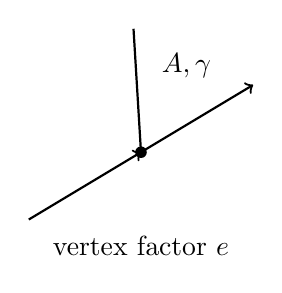
\begin{tikzpicture}[scale=0.95]
\draw[thick,->] (-1.5,-0.9) -- (0,0);
\draw[thick,->] (0,0) -- (1.5,0.9);
\draw[thick] (0,0) -- (-0.1,1.65);
\fill (0,0) circle (2.2pt);
\node[right] at (0.15,1.15) {$A,\gamma$};
\node at (0,-1.25) {vertex factor $e$};
\end{tikzpicture}
\caption{Đỉnh electron--electron--photon sơ cấp của điện động lực học lượng tử.}
\end{figure}

\begin{classroomqa}
\lecturetimestamp{01:27:38}
\audiencequestion{Còn tán xạ electron--proton thì sao?}
\lecturerresponse{Trong cách xử lý nguyên tử sơ cấp, proton có thể được lý tưởng hóa như một nguồn điểm cố định, nặng vô hạn---một hạt nặng bị ghim chặt tại chỗ. Động lực học trường lượng tử của bản thân nó chỉ xuất hiện khi đưa vào lý thuyết nội tại của proton và neutron.}
\end{classroomqa}

\begin{classroomqa}
\lecturetimestamp{01:28:30}
\audiencequestion{Electron có thể chuyển động gần bằng tốc độ ánh sáng so với proton đó không?}
\lecturerresponse{Có.}
\end{classroomqa}

Hãy xét photon tán xạ trên một electron. Ở bậc thấp nhất, đồ thị có hai đỉnh electron--electron--photon. Vì vậy biên độ tỉ lệ với \(e^2\):
\begin{equation}
\mathcal{A}_{\mathrm{lowest}}\propto e^2.
\end{equation}
Xác suất, hay tương đương là sự phụ thuộc theo hằng số liên kết của tiết diện tán xạ, đến từ bình phương môđun và tỉ lệ với \(e^4\):
\begin{equation}
P_{\mathrm{lowest}}\ \text{or}\ \sigma_{\mathrm{lowest}}
\propto e^4.
\end{equation}
Với chuẩn hóa không thứ nguyên thông thường, liên kết điện là nhỏ, nên tán xạ thực sự ít có khả năng xảy ra hơn nhiều so với việc photon đơn giản đi qua mà không tán xạ.

Ngay ở bậc này đã có hai đồ thị. Trong một thứ tự, photon tới bị hấp thụ và photon ra được phát ra sau đó. Trong thứ tự kia, photon ra được phát ra trước khi photon tới bị hấp thụ. Cả hai biên độ đều đóng góp.\footnote{Hai thứ tự theo thời gian được dựng lại từ các giản đồ tại 01:28:42 và 01:30:18.}

\begin{figure}[htbp]
\centering
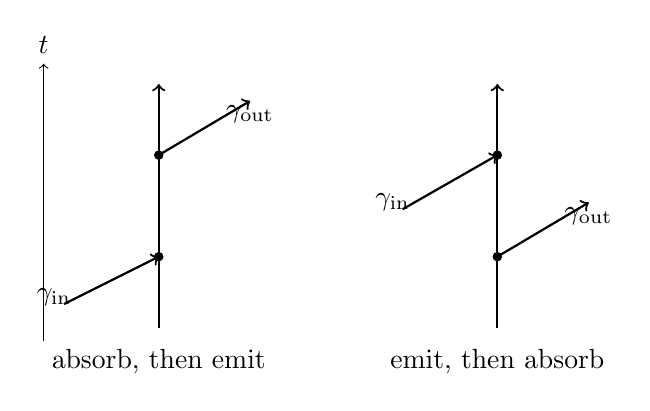
\begin{tikzpicture}[scale=0.86]
\draw[->] (-0.7,0) -- (-0.7,4.1) node[above] {$t$};
\draw[thick,->] (1.0,0.2) -- (1.0,3.8);
\fill (1.0,1.25) circle (2pt);
\fill (1.0,2.75) circle (2pt);
\draw[thick,->] (-0.4,0.55) -- (1.0,1.25);
\draw[thick,->] (1.0,2.75) -- (2.35,3.55);
\node[left] at (-0.15,0.65) {$\gamma_{\mathrm{in}}$};
\node[right] at (1.85,3.35) {$\gamma_{\mathrm{out}}$};
\node at (1.0,-0.3) {absorb, then emit};
\begin{scope}[xshift=5.0cm]
\draw[thick,->] (1.0,0.2) -- (1.0,3.8);
\fill (1.0,1.25) circle (2pt);
\fill (1.0,2.75) circle (2pt);
\draw[thick,->] (1.0,1.25) -- (2.35,2.05);
\draw[thick,->] (-0.4,1.95) -- (1.0,2.75);
\node[right] at (1.85,1.85) {$\gamma_{\mathrm{out}}$};
\node[left] at (-0.15,2.05) {$\gamma_{\mathrm{in}}$};
\node at (1.0,-0.3) {emit, then absorb};
\end{scope}
\end{tikzpicture}
\caption{Hai thứ tự theo thời gian bậc thấp nhất cho tán xạ electron--photon.}
\end{figure}

Do đó, biên độ bậc thấp nhất không phải là một đồ thị mà là tổng của hai đồ thị:
\begin{equation}
\begin{aligned}
\mathcal{A}^{(2)}
&=
\mathcal{A}_{\mathrm{absorb\ then\ emit}}
+\mathcal{A}_{\mathrm{emit\ then\ absorb}},\\
\mathcal{A}^{(2)}&\propto e^2.
\end{aligned}
\end{equation}

Các hiệu chỉnh bậc cao hơn bổ sung thêm các đỉnh sơ cấp. Một photon nội bộ bổ sung gắn hai lần vào đường electron sẽ thêm hai thừa số \(e\), cho một đóng góp tỉ lệ với \(e^4\) trong biên độ và \(e^8\) trong bình phương độ lớn của nó. Một đường photon cũng có thể chứa một chèn electron--positron, lại thêm các đỉnh sơ cấp và các lũy thừa bổ sung của \(e\). Đây là các ví dụ, không phải danh sách đầy đủ; photon thêm vào có thể được gắn ở nhiều vị trí.\footnote{Các cấu trúc bậc cao hơn được dựng lại từ 01:30:38--01:31:16.}

\begin{figure}[htbp]
\centering
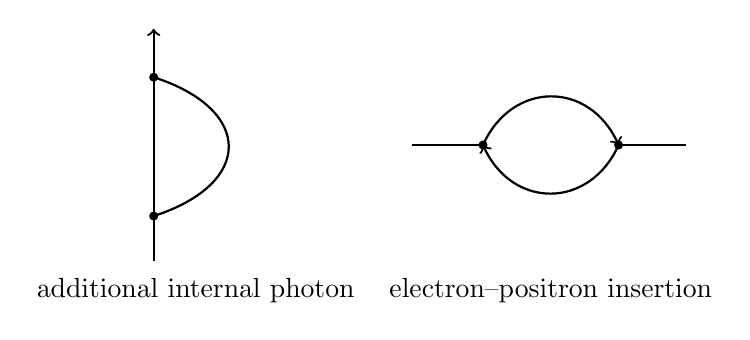
\begin{tikzpicture}[scale=0.82]
\draw[thick,->] (0.9,0.2) -- (0.9,3.8);
\fill (0.9,0.9) circle (2pt);
\fill (0.9,3.05) circle (2pt);
\draw[thick] (0.9,0.9) .. controls (2.45,1.4) and (2.45,2.55) .. (0.9,3.05);
\node at (1.55,-0.25) {additional internal photon};
\begin{scope}[xshift=5.1cm]
\draw[thick] (-0.2,2.0) -- (0.9,2.0);
\fill (0.9,2.0) circle (2pt);
\fill (3.0,2.0) circle (2pt);
\draw[thick,->] (0.9,2.0) .. controls (1.35,3.0) and (2.55,3.0) .. (3.0,2.0);
\draw[thick,->] (3.0,2.0) .. controls (2.55,1.0) and (1.35,1.0) .. (0.9,2.0);
\draw[thick] (3.0,2.0) -- (4.05,2.0);
\node at (1.95,-0.25) {electron--positron insertion};
\end{scope}
\end{tikzpicture}
\caption{Hai cấu trúc QED bậc cao hơn thêm các đỉnh sơ cấp và các lũy thừa tiếp theo của \(e\).}
\end{figure}

Vì vậy khai triển QED tiến hành theo các lũy thừa kế tiếp của \(e^2\). Mỗi mức phức tạp mới cùng loại thêm hai lũy thừa của điện tích vào biên độ. Trong chuẩn hóa đang dùng, điều đó khiến một hiệu chỉnh như vậy có biên độ nhỏ hơn bậc trước chừng một trăm hoặc vài trăm lần. Các đồ thị phức tạp hơn yếu dần đi, nên tổng nhiễu loạn có cơ may trở nên hữu ích.

Xác suất không được thu bằng cách bình phương riêng từng đồ thị rồi cộng các bình phương ấy lại. Trước hết hãy cộng mọi biên độ đóng góp vào cùng một quá trình với cùng các hạt ngoài:
\begin{equation}
\mathcal{A}_{\mathrm{total}}=\sum_r\mathcal{A}_r.
\end{equation}
Chỉ sau đó mới lập
\begin{equation}
P=\left|\mathcal{A}_{\mathrm{total}}\right|^2
=\left|\sum_r\mathcal{A}_r\right|^2.
\end{equation}
Các hạng chéo giữa những đồ thị khác nhau là các hạng giao thoa. Quy tắc thì đơn giản và thiết yếu: cộng trước, rồi mới bình phương.

\section{Hướng tới danh mục hạt và Mô hình Chuẩn}

Khi đã có hàm truyền, đỉnh, cách đếm theo hằng số liên kết và giao thoa, việc mô tả vật lý hạt có thể thực sự bắt đầu. Ta có thể gọi tên các hạt, chỉ rõ khối lượng của chúng, viết các Lagrangian chi phối chúng một phần từ lý thuyết và một phần từ thực nghiệm, rồi nghiên cứu trực tiếp các đối xứng của chúng ngay trong các Lagrangian ấy. Chính khuôn khổ đó sau đó dẫn tới Mô hình Chuẩn và các tính chất của nó.

\begin{classroomqa}
\lecturetimestamp{01:33:22}
\audiencequestion{Liệu hệ số khối lượng không đổi \(m^2\) có thể được thay bằng trường Higgs không?}
\lecturerresponse{Có. Đó là ý tưởng đúng, và cơ chế ấy sẽ được bàn sau.}
\end{classroomqa}

\begin{classroomqa}
\lecturetimestamp{01:33:42}
\audiencequestion{Hai điểm mạng lân cận \(x\) và \(x'\) có thể nằm ở hai thời điểm khác nhau không?}
\lecturerresponse{Có. Chúng có thể là lân cận theo hướng thời gian; đó là cách sự truyền thẳng đứng trên mạng được biểu diễn.}
\end{classroomqa}

Đối với các điểm lân cận, bình phương sai phân hữu hạn chứa cả các hạng cùng điểm mạng lẫn các hạng liên kết chéo:
\begin{equation}
\bigl[\phi(x)-\phi(x')\bigr]^2
=
\phi(x)^2+\phi(x')^2-2\phi(x)\phi(x').
\end{equation}

\begin{classroomqa}
\lecturetimestamp{01:33:56}
\audiencequestion{Hạng nào biểu diễn một hạt chỉ đơn giản đứng yên?}
\lecturerresponse{Các hạng cùng điểm \(\phi(x)^2\) và \(\phi(x')^2\) trong bình phương sai phân hữu hạn biểu diễn việc đứng yên, còn hạng chéo \(\phi(x)\phi(x')\) đem lại cách diễn giải chuyển động. Hạng khối lượng tường minh cũng đóng góp các thừa số cùng điểm, tương ứng với đứng yên.}
\end{classroomqa}